\chapter{Superspace et construction de la dynamique supersymétrique}

\lectureoverview{Nous reconstruisons la supersymétrie à partir du système le plus simple sur lequel elle peut agir : un oscillateur bosonique et un oscillateur fermionique de même énergie. Le contraste entre leurs équations du deuxième et du premier ordre conduit aux charges supersymétriques et à leur algèbre. Nous réinterprétons ensuite cette algèbre comme une géométrie sur un espace muni de la coordonnée ordinaire (t) et des coordonnées de Grassmann \(\theta,\bar\theta\). Les superchamps réunissent les bosons, les fermions et un champ auxiliaire en un seul objet ; l’intégration de Berezin extrait un lagrangien ordinaire invariant ; les dérivées covariantes permettent d’imposer des contraintes compatibles avec la symétrie ; et la contrainte chirale en fournit le premier exemple important. Le cours met délibérément en évidence les difficultés liées aux signes et à l’ordre des facteurs dans ce formalisme, puis s’achève en expliquant pourquoi la symétrie elle-même est plus fondamentale qu’un catalogue de règles de Feynman.}

\section{Retour au système à un seul mode}

Repartons des fermions et des bosons au repos. Nous supprimons toutes les coordonnées spatiales et tous les indices de quantité de mouvement. Dans un mode donné, un quantum est présent ou absent ; les opérateurs de création et d’annihilation suffisent à le décrire. Notons \(a^\dagger,a\) un mode bosonique et \(c^\dagger,c\) un mode fermionique. Ils vérifient
\begin{align}
[a,a^\dagger]&=1,
&
\{c,c^\dagger\}&=1,
&
c^2=(c^\dagger)^2&=0.
\end{align}
Si les deux quanta ont la même énergie \(m\), alors, à une constante de vide sans importance près,
\begin{equation}
H=m\left(a^\dagger a+c^\dagger c\right).
\label{eq:l7-one-mode-hamiltonian}
\end{equation}
L’opérateur nombre \(a^\dagger a\) peut prendre toute valeur entière non négative, tandis que \(c^\dagger c\) ne peut valoir que zéro ou un. Toute la cinématique de ce modèle jouet se résume à cela.

Cette simplification est stratégique. Nous voulons comprendre l’opération qui élimine un boson et crée un fermion, ou fait l’inverse, sans modifier l’énergie. Avant de construire cette opération, traduisons toutefois le même système du langage des opérateurs en langage lagrangien.

\section{L’oscillateur bosonique}

Pour le boson, introduisons une coordonnée réelle \(\phi(t)\). En l’absence de variation spatiale, un champ scalaire libre devient un oscillateur harmonique ordinaire. La première expression écrite au tableau était
\[
\frac{1}{2}\dot\phi^{,2}+\frac{1}{2}m^2\phi^2.
\]
Cette expression est l’énergie cinétique plus l’énergie potentielle, et non le lagrangien. Le cours corrige aussitôt le signe :
\begin{equation}
L_B=\frac{1}{2}\dot\phi^{,2}-\frac{1}{2}m^2\phi^2.
\label{eq:l7-boson-lagrangian}
\end{equation}

\begin{figure}[H]
\centering
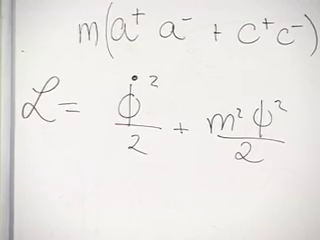
\includegraphics[width=0.62\textwidth]{lecture_07_figure_02.png}
\lectureframe{00:03:25.431}
\caption{L’hamiltonien à un mode au-dessus du lagrangien bosonique. L’image conserve le signe plus initial avant la correction formulée à l’oral vers \(T-V\).}
\end{figure}

\begin{classroomqa}
\audiencequestion{Qu’est-ce qui ne va pas dans le signe du lagrangien de l’oscillateur affiché ? \lecturetimestamp{00:04:00}}
\lecturerresponse{L’énergie est \(T+V\), mais le lagrangien est \(T-V\). Le terme de potentiel doit donc porter un signe moins. Cette correction remplace le comportement exponentiel par l’oscillation harmonique attendue.}
\end{classroomqa}

En effet, l’équation d’Euler--Lagrange donne
\begin{align}
\frac{d}{dt}\frac{\partial L_B}{\partial\dot\phi}
&=\frac{\partial L_B}{\partial\phi},\\
\ddot\phi&=-m^2\phi,
\end{align}ou
\begin{equation}
\ddot\phi+m^2\phi=0.
\label{eq:l7-boson-eom}
\end{equation}
Sa fréquence est \(m\), et non \(m^2\). La quantification de cet oscillateur produit la même échelle d’états que celle décrite par \(a^\dagger\) et \(a\) dans l’équation~\eqref{eq:l7-one-mode-hamiltonian}.

\section{Pourquoi l’action fermionique est du premier ordre}

Le lagrangien fermionique paraît plus simple parce qu’il ne contient qu’une dérivée temporelle. On en voit déjà la raison dans un essai délibérément naïf. Pour une variable ordinaire commutative,
\begin{equation}
L_{\mathrm{trial}}=\phi\dot\phi
=\frac{1}{2}\frac{d}{dt}\phi^2.
\end{equation}
C’est une dérivée totale. Son équation d’Euler--Lagrange indique seulement \(\dot\phi=\dot\phi\), de sorte que toute trajectoire différentiable est permise. Soustraire une dérivée totale à l’action modifie les données aux extrémités, mais pas l’équation du mouvement dans le volume.

Renommons maintenant la variable \(\psi\) et déclarons-la impaire de Grassmann. \(\psi\) et \(\dot\psi\) anticommutent. Avec un choix fixé de variation à gauche, la permutation des facteurs impairs introduit un signe moins ; le même essai formel donne donc
\begin{equation}
\frac{d}{dt}\frac{\partial L_{\mathrm{trial}}}{\partial\dot\psi}
=\dot\psi,
\qquad
\frac{\partial L_{\mathrm{trial}}}{\partial\psi}
=-\dot\psi.
\end{equation}
L’équation est alors
\begin{equation}
\dot\psi=-\dot\psi
\quad\Longrightarrow\quad
\dot\psi=0.
\label{eq:l7-constant-fermion}
\end{equation}
L’expression qui était une tautologie pour une coordonnée commutative acquiert un contenu dynamique pour une variable anticommutative. Ce contenu est trop contraignant pour un oscillateur, puisqu’il n’autorise qu’une constante, mais c’est précisément l’indice dont nous avons besoin.

\begin{classroomqa}
\audiencequestion{La solution consiste-t-elle simplement à dire que \(\psi\) est constante ? \lecturetimestamp{00:13:57}}
\lecturerresponse{Oui. L’équation~\eqref{eq:l7-constant-fermion} est une véritable équation différentielle du premier ordre, dont la solution est une constante arbitraire à valeurs de Grassmann. Un terme de masse transformera cette solution statique en une solution oscillante.}
\end{classroomqa}

La tentative évidente, \(m\psi^2\), échoue parce que \(\psi^2=0\). Il nous faut deux variables réelles impaires \(\psi_1,\psi_2\), ou, de manière équivalente, une variable complexe et sa conjuguée. Le cours développe au tableau la formulation à deux variables réelles, en vérifiant à plusieurs reprises les signes et les facteurs de deux. Une formulation complexe normalisée selon la convention usuelle est
\begin{equation}
L_F=\frac{i}{2}
\left(\bar\psi\dot\psi-\dot{\bar\psi}\psi\right)
-m\bar\psi\psi.
\label{eq:l7-fermion-lagrangian}
\end{equation}
À une dérivée totale près, cela donne \(i\bar\psi\dot\psi-m\bar\psi\psi\). La variation par rapport à \(\bar\psi\) donne
\begin{equation}
i\dot\psi=m\psi,
\qquad
\psi(t)=\psi(0)e^{-imt}.
\label{eq:l7-fermion-eom}
\end{equation}
L’équation conjuguée a une phase opposée. Le mode fermionique oscille donc avec l’énergie \(m\), comme le mode bosonique, bien que son équation soit du premier ordre et non du deuxième.

\editorialnote{L’équation~\eqref{eq:l7-fermion-lagrangian} fixe un ordre et une normalisation standard pour le calcul exploratoire à deux variables réelles. Dans le cours, le facteur \(i\) est inséré, un facteur deux est ajusté et le signe d’une composante réelle reste indéterminé. Ces changements ne modifient pas la conclusion centrale : la cinétique des fermions est du premier ordre, la masse intervient linéairement et un fermion complexe fournit un bilinéaire non nul.}

C’est l’ombre, en dimension zéro, d’un contraste relativiste bien connu. L’équation de Klein--Gordon est du deuxième ordre en temps, tandis que l’équation de Dirac est du premier ordre. Lorsque l’on supprime les coordonnées spatiales, le boson devient un oscillateur harmonique et le fermion, un oscillateur complexe de Grassmann.

\begin{classroomqa}
\audiencequestion{L’ordre dans lequel on écrit \(\psi\), \(\dot\psi\) et leurs conjugués a-t-il de l’importance ? \lecturetimestamp{00:18:58}}
\lecturerresponse{Les formules intermédiaires dépendent bien de l’ordre, car les facteurs impairs anticommutent. La théorie physique ne dépend pas d’un choix arbitraire de notation, à condition d’appliquer partout une même convention pour les variations à gauche ou à droite, la conjugaison et l’intégration. Inverser l’ordre de deux facteurs impairs change un signe ; il faut alors modifier de manière cohérente tous les autres signes concernés.}
\end{classroomqa}

En combinant les équations~\eqref{eq:l7-boson-lagrangian} et \eqref{eq:l7-fermion-lagrangian}, on obtient une description lagrangienne de la même paire appariée que celle représentée par l’équation~\eqref{eq:l7-one-mode-hamiltonian}. Nous pouvons maintenant identifier la symétrie qui les relie.

\section{Les charges supersymétriques et leur algèbre}

Un opérateur qui élimine un fermion et crée un boson est
\begin{equation}
Q^\dagger=\sqrt{2m}\,a^\dagger c,
\end{equation}
tandis que son conjugué élimine un boson et crée un fermion,
\begin{equation}
Q=\sqrt{2m}\,a c^\dagger.
\end{equation}
La normalisation est choisie de façon à obtenir la forme standard de l’algèbre. En utilisant \(cc^\dagger=1-c^\dagger c\), \(aa^\dagger=a^\dagger a+1\) et le fait que les opérateurs bosoniques commutent avec les opérateurs fermioniques,
\begin{align}
\{Q,Q^\dagger\}
&=2m\left(ac^\dagger a^\dagger c+a^\dagger c a c^\dagger\right)\notag\\
&=2m\left[(a^\dagger a+1)c^\dagger c
+a^\dagger a(1-c^\dagger c)\right]\notag\\
&=2m\left(a^\dagger a+c^\dagger c\right)=2H.
\label{eq:l7-superalgebra}
\end{align}
On peut déplacer les opérateurs bosoniques au travers des opérateurs fermioniques. La même nilpotence qui limite l’occupation fermionique donne
\begin{equation}
Q^2=(Q^\dagger)^2=0.
\end{equation}
Enfin,
\begin{equation}
[H,Q]=[H,Q^\dagger]=0.
\label{eq:l7-conserved-supercharges}
\end{equation}
Chaque charge supersymétrique modifie le nombre de bosons et le nombre de fermions en sens opposés ; les deux variations d’énergie s’annulent donc lorsque les fréquences sont égales.

\begin{classroomqa}
\audiencequestion{Que vaut \([H,Q]\) ? La réponse est-elle proportionnelle à \(Q\) ? \lecturetimestamp{00:25:10}}
\lecturerresponse{Non. La réponse est zéro. Un opérateur de création ou d’annihilation isolé acquiert son énergie lorsqu’on le commute avec \(H\), mais les contributions bosonique et fermionique dans \(Q\) s’annulent. Cette annulation est précisément la condition d’égalité des énergies.}
\end{classroomqa}

\begin{classroomqa}
\audiencequestion{Cette relation de commutation n’avait-elle pas déjà été écrite au tableau ? \lecturetimestamp{00:25:45}}
\lecturerresponse{Si. La redécouvrir est utile, car cela nous oblige à interpréter la relation plutôt qu’à la recopier : commuter avec l’hamiltonien signifie que la transformation est une symétrie et que son générateur est conservé.}
\end{classroomqa}

Le qualificatif \emph{charge} renvoie à cette loi de conservation. Il ne faut toutefois pas considérer \(Q\) comme un nombre ordinaire, mesurable simultanément, associé à un état. Cette quantité est impaire de Grassmann, nilpotente et transforme un état bosonique en état fermionique. L’énoncé utile est qu’il s’agit d’un générateur conservé qui agit au sein de supermultiplets dégénérés.
\editorialnote{Cette formulation précise l’analogie faite en cours avec la classification des états par leur énergie ou leur charge électrique. Les charges supersymétriques impaires, prises individuellement et non hermitiennes, ne sont pas des observables ordinaires auxquelles correspondent des nombres quantiques. C’est leur action conservée et la représentation de l’ensemble de la superalgèbre qui fournissent la classification correcte.}

\section{Les générateurs comme dérivées}

L’algèbre est compacte, mais elle ne nous indique pas à elle seule comment construire des théories avec interactions. L’étape suivante est géométrique. Les générateurs des symétries usuelles agissent déjà comme des opérateurs différentiels. Dans la convention du cours,
\begin{equation}
H=i\frac{\partial}{\partial t},
\qquad
P=-i\frac{\partial}{\partial x}.
\end{equation}

\begin{figure}[H]
\centering
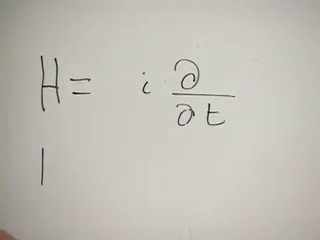
\includegraphics[width=0.50\textwidth]{lecture_07_figure_03.png}
\lectureframe{00:28:12.720}
\caption{L’hamiltonien représenté comme générateur des translations temporelles.}
\end{figure}

Le moment cinétique est lui aussi un produit d’une coordonnée et d’une dérivée. Si les charges supersymétriques sont des générateurs impairs, on peut naturellement se demander si elles peuvent être représentées par des dérivées par rapport à des coordonnées impaires. Nous étendons donc l’axe temporel en le remplaçant par le superspace
\begin{equation}
(t,\theta,\bar\theta),
\qquad
\theta^2=\bar\theta^2=0,
\qquad
\theta\bar\theta=-\bar\theta\theta.
\end{equation}
Les champs sur cet espace dépendent du temps ordinaire et d’une paire conjuguée de coordonnées de Grassmann.

Le cours montre délibérément à quel point les signes sont délicats. Le signe provenant de la conjugaison complexe, celui provenant du déplacement d’un paramètre impair et celui qui découle du choix de dérivées à gauche plutôt qu’à droite correspondent à des opérations différentes. Au lieu de conserver des étapes au tableau mutuellement incompatibles, fixons une convention : toutes les dérivées impaires sont des dérivées à gauche, et
\begin{equation}
q=\partial_\theta+i\bar\theta\partial_t,
\qquad
\bar q=\partial_{\bar\theta}+i\theta\partial_t.
\label{eq:l7-differential-supercharges}
\end{equation}
Alors
\begin{equation}
q^2=\bar q^{,2}=0,
\qquad
\{q,\bar q\}=2i\partial_t=2H.
\label{eq:l7-differential-algebra}
\end{equation}
Le facteur deux provient de deux termes croisés : \(\{\partial_\theta,\theta\}=1\) et \(\{\partial_{\bar\theta},\bar\theta\}=1\). Si les générateurs ne contenaient que \(\partial_\theta\) et \(\partial_{\bar\theta}\), leur anticommutateur s’annulerait et ne pourrait pas reproduire l’hamiltonien.

\begin{classroomqa}
\audiencequestion{Les deux termes de dérivée temporelle dans \(q\) et \(\bar q\) doivent-ils avoir le même signe ? \lecturetimestamp{00:31:01}}
\lecturerresponse{Il faut choisir leurs signes de manière cohérente afin que l’anticommutateur mixte soit \(2H\). On peut adopter une convention avec un signe plus global, ou l’alternative conjuguée de manière cohérente. C’est le calcul, et non l’intuition visuelle associée au symbole \(i\), qui fixe les signes relatifs.}
\end{classroomqa}

Dans la salle, les signes sont vérifiés à plusieurs reprises, et leur difficulté devient un sujet de plaisanterie : ils semblent changer pendant le trajet pour aller travailler. La plaisanterie est bien trouvée. Faire passer un paramètre de Grassmann au travers d’une coordonnée peut changer un signe, même si aucune convention physique n’a changé. L’équation~\eqref{eq:l7-differential-supercharges} est la référence fixe pour tout ce qui suit.

\subsection{La supersymétrie comme déplacement de coordonnées}

Soient \(\xi,\bar\xi\) des paramètres impairs infinitésimaux. L’action sur un superchamp de
\begin{equation}
\delta_\xi=\xi q+\bar\xi\bar q
\end{equation}
équivaut, dans la convention ci-dessus, au changement infinitésimal de coordonnées
\begin{align}
\theta&\longrightarrow\theta+\xi,\\
\bar\theta&\longrightarrow\bar\theta+\bar\xi,\\
t&\longrightarrow t+i\left(\xi\bar\theta+\bar\xi\theta\right).
\label{eq:l7-coordinate-shift}
\end{align}
La variation d’un superchamp scalaire est donc
\begin{equation}
\delta_\xi\Phi
=\left(\xi\partial_\theta+\bar\xi\partial_{\bar\theta}
+i\xi\bar\theta\partial_t+i\bar\xi\theta\partial_t\right)\Phi
=\left(\xi q+\bar\xi\bar q\right)\Phi.
\end{equation}
Voilà le contenu géométrique de la supersymétrie. Il s’agit d’une translation dans les directions impaires, liée à une translation du temps ordinaire. La composition de deux déplacements impairs donne une translation temporelle, conformément à l’équation~\eqref{eq:l7-differential-algebra}.

\begin{classroomqa}
\audiencequestion{Le signe moins contesté pourrait-il représenter un déplacement vers le passé ? \lecturetimestamp{00:58:13}}
\lecturerresponse{Une convention différente pour les signes peut inverser le déplacement temporel infinitésimal affiché, mais elle n’introduit aucun processus physique distinct de retour dans le temps. L’essentiel est que la transformation des coordonnées et les générateurs différentiels obéissent à la même algèbre.}
\end{classroomqa}

\begin{classroomqa}
\audiencequestion{Ce temps étendu a-t-il une réalisation physique, ou s’agit-il seulement d’un artifice de calcul ? \lecturetimestamp{00:58:23}}
\lecturerresponse{C’est un artifice de calcul en un sens utile : il intègre l’algèbre à une géométrie. Mais cet artifice devient physiquement précieux lorsqu’on introduit des interactions. Le superspace fournit un calcul systématique pour construire des lagrangiens qui préservent à chaque étape la symétrie boson--fermion, tout comme le calcul tensoriel aide à construire des scalaires de Lorentz.}
\end{classroomqa}

\section{Superchamps et composante auxiliaire}

Comme il n’y a que deux coordonnées impaires, le développement d’un superchamp pair s’arrête :
\begin{equation}
\Phi(t,\theta,\bar\theta)
=\phi(t)+\bar\theta\psi(t)+\bar\psi(t)\theta
+D(t)\bar\theta\theta.
\label{eq:l7-superfield}
\end{equation}
Les coefficients des monômes pairs, \(\phi\) et \(D\), sont bosoniques ; ceux des monômes impairs, \(\psi\) et \(\bar\psi\), sont fermioniques. Aucun terme \(\theta^2\), \(\bar\theta^2\) ou d’ordre supérieur ne subsiste. Nous ne développons pas la dépendance temporelle, car un développement de Taylor ordinaire en \(t\) ne s’arrêterait pas et serait sans utilité ici.

\begin{classroomqa}
\audiencequestion{Que représente la composante \(D(t)\) dans le terme de plus haut degré ? \lecturetimestamp{00:41:46}}
\lecturerresponse{À ce stade, il s’agit simplement du dernier coefficient bosonique dans le développement fini. Dans l’action en composantes, elle n’a généralement pas de terme cinétique et est éliminée par une équation du mouvement algébrique ; on l’appelle donc champ auxiliaire. Le cours propose sur le ton de la plaisanterie ``D pour dummy (auxiliaire),'' ce qui décrit son rôle non dynamique sans pour autant constituer l’origine historique de cette appellation.}
\end{classroomqa}

Le superchamp est un objet unique, tandis que \(\phi,\psi,\bar\psi,D\) en sont les composantes. Une transformation supersymétrique les mélange. Un boson et un fermion sont donc reliés selon une structure très semblable à celle qui relie, par une rotation, les composantes selon \(x\) et \(y\) d’un vecteur, même si les directions de Grassmann ne peuvent pas être représentées comme des axes ordinaires.

\section{La superaction et la composante de plus haut degré}

Pour obtenir les équations du mouvement, il nous faut une action. En théorie des champs ordinaire, on forme un lagrangien scalaire et on l’intègre sur l’espace-temps. Ici, l’expression analogue est
\begin{equation}
S=\int dt\,d\theta\,d\bar\theta\;\Lambda
\bigl(\Phi,\text{ superspace derivatives of }\Phi\bigr),
\label{eq:l7-superaction}
\end{equation}
où \(\Lambda\) est un superchamp pair. L’intégration de Berezin est algébrique. Choisissons
\begin{equation}
\int d\theta\,d\bar\theta\;\bar\theta\theta=1.
\end{equation}
Par conséquent, si
\begin{equation}
\Lambda=A+\bar\theta B+\bar B\theta+C\bar\theta\theta,
\end{equation}
alors
\begin{equation}
\int d\theta\,d\bar\theta\;\Lambda=C.
\label{eq:l7-top-component}
\end{equation}
L’intégration sur les variables impaires extrait la composante de plus haut degré et laisse un lagrangien ordinaire à intégrer sur le temps.

Pourquoi le résultat est-il invariant ? Une variation supersymétrique translate les variables d’intégration. La variation de la composante de plus haut degré est une dérivée totale ordinaire par rapport au temps, tandis que les dérivées totales impaires s’annulent dans l’intégration de Berezin. Sous des conditions convenables aux extrémités, l’action reste inchangée. C’est l’analogue, dans le superspace, de la construction d’un scalaire de Lorentz avant son intégration sur l’espace-temps.

\section{Multiplication de superchamps}

Le moyen le plus simple de construire un nouveau superchamp à partir d’un autre est de le multiplier par lui-même. En partant de l’équation~\eqref{eq:l7-superfield}, tous les termes contenant \(\theta^2\) ou \(\bar\theta^2\) s’annulent. En conservant l’ordre \(\bar\theta\theta\) et en plaçant à gauche les champs composantes barrés, on obtient
\begin{align}
\Phi^2
={}&\phi^2
+2\phi\bar\theta\psi
+2\phi\bar\psi\theta\notag\\
&+\left(2\phi D-2\bar\psi\psi\right)\bar\theta\theta.
\label{eq:l7-superfield-square}
\end{align}

\begin{figure}[H]
\centering
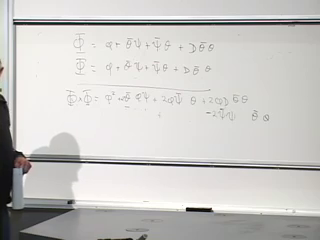
\includegraphics[width=0.82\textwidth]{lecture_07_figure_05.png}
\lectureframe{01:07:57.844}
\caption{Le produit de superchamps, développé composante par composante, et l’ensemble de ses termes en \(\bar\theta\theta\).}
\end{figure}

Les deux termes \(\phi D\) et \(D\phi\) s’additionnent parce que les deux champs sont pairs. Les deux termes croisés fermioniques s’additionnent également après permutation de leurs facteurs, mais leur signe commun est négatif :
\begin{equation}
(\bar\theta\psi)(\bar\psi\theta)
+(\bar\psi\theta)(\bar\theta\psi)
=-2\bar\psi\psi\,\bar\theta\theta.
\end{equation}
L’intégration du carré sur les coordonnées impaires donne
\begin{equation}
\int d\theta\,d\bar\theta\;\Phi^2
=2\phi D-2\bar\psi\psi.
\end{equation}
Ce terme est supersymétrique par construction, mais ce n’est pas encore un lagrangien cinétique. Il ne contient aucune dérivée temporelle.

Le cours propose ensuite \(\Phi^3\), \(\Phi^4\) et \(\Phi^n\) comme exercices. Il existe une règle compacte. Pour toute fonction ordinaire \(W\),
\begin{equation}
\left.W(\Phi)\right|_{\bar\theta\theta}
=W'(\phi)D-W''(\phi)\bar\psi\psi.
\label{eq:l7-function-top-component}
\end{equation}
Pour \(W(\phi)=\phi^2\), on retrouve l’équation~\eqref{eq:l7-superfield-square} ; pour \(W(\phi)=\phi^n\), on obtient
\begin{equation}
\left.\Phi^n\right|_{\bar\theta\theta}
=n\phi^{n-1}D-n(n-1)\phi^{n-2}\bar\psi\psi.
\end{equation}
\editorialnote{Le cours donne comme exercice la puissance \(n\) et indique les types de termes attendus. L’équation~\eqref{eq:l7-function-top-component} fournit la règle complète selon la convention d’ordre fixée.}

À ce stade, l’enseignant demande à la salle si elle est épuisée. Le public répond que non ; il répond, lui, qu’il l’est. Cet échange ne sert pas seulement de détente comique. Les puissances de superchamps sont simples, car le développement s’arrête, mais les dérivées et les contraintes sont là où le suivi des signes devient réellement exigeant.

\section{Quelles dérivées respectent la supersymétrie ?}

Il faut corriger un point avant de suivre l’argument suivant au tableau. La dérivée temporelle ordinaire ne pose pas de problème :
\begin{equation}
[\partial_t,q]=[\partial_t,\bar q]=0.
\end{equation}
Par conséquent, \(\partial_t\Phi\) se transforme comme un superchamp dès lors que \(\Phi\) le fait. Les objets subtils sont les dérivées impaires brutes \(\partial_\theta\Phi\) et \(\partial_{\bar\theta}\Phi\), car elles n’anticommutent pas avec les deux charges supersymétriques. Il nous faut des dérivées impaires modifiées pour les contraintes et pour construire des composantes manifestement supersymétriques.
\editorialnote{L’affirmation orale selon laquelle une dérivation temporelle ne produit pas un autre superchamp est incorrecte dans la convention utilisée ici. Puisque \(\partial_t\) commute avec les deux charges supersymétriques, elle est covariante. La construction ultérieure de dérivées impaires modifiées reste nécessaire et constitue le véritable point mathématique du cours.}

\subsection{L’analogie du champ ``magique''}

Le cours motive ce critère par l’exemple des rotations ordinaires. Soit \(f(x,y)\) une fonction vérifiant
\begin{equation}
\partial_y f=0.
\label{eq:l7-magic-constraint}
\end{equation}
Appelons une telle fonction un « champ ``magique'' ». Elle dépend de \(x\), mais pas de \(y\). La classe des champs magiques est-elle préservée par les rotations ? Pour
\begin{equation}
L_z=-i\left(x\partial_y-y\partial_x\right),
\end{equation}
on trouve
\begin{equation}
[\partial_y,L_z]=i\partial_x\neq0.
\end{equation}
Par conséquent, \(L_z f\) acquiert en général une dépendance en \(y\), même lorsque \(f\) vérifie initialement l’équation~\eqref{eq:l7-magic-constraint}. La contrainte n’est pas invariante par rotation.

La leçon générale est simple. Si un champ vérifie \(C\Phi=0\) et si une symétrie est engendrée par \(G\), le champ transformé reste contraint lorsque le commutateur gradué de \(C\) avec \(G\) s’annule. Pour deux opérateurs impairs, le commutateur gradué est un anticommutateur.

\begin{classroomqa}
\audiencequestion{Quand une contrainte imposée à un champ est-elle compatible avec une symétrie ? \lecturetimestamp{01:17:56}}
\lecturerresponse{Lorsque l’opérateur de contrainte commute au sens gradué avec les générateurs de la symétrie. On peut alors faire passer \(C(G\Phi)\) au travers de \(G\) et retrouver \(G(C\Phi)=0\). L’exemple des rotations échoue parce que \(\partial_y\) ne commute pas avec le générateur de rotation.}
\end{classroomqa}

\subsection{Dérivées impaires covariantes}

Les charges supersymétriques étant fixées par l’équation~\eqref{eq:l7-differential-supercharges}, définissons
\begin{equation}
\mathcal D=\partial_\theta-i\bar\theta\partial_t,
\qquad
\bar{\mathcal D}=\partial_{\bar\theta}-i\theta\partial_t.
\label{eq:l7-covariant-derivatives}
\end{equation}
Seul le signe du terme de dérivée temporelle change. Un calcul direct donne
\begin{align}
\{\mathcal D,q\}
&=\{\mathcal D,\bar q\}
=\{\bar{\mathcal D},q\}
=\{\bar{\mathcal D},\bar q\}=0,\\
\{\mathcal D,\bar{\mathcal D}\}&=-2i\partial_t.
\label{eq:l7-covariant-algebra}
\end{align}
Les deux termes croisés potentiellement non nuls s’annulent. C’est l’analogue impair d’une dérivée covariante : elle dérive tout en préservant la loi de transformation.

Le cours utilise \(D\) à la fois pour la composante auxiliaire et pour cette dérivée. Nous réservons \(D(t)\) à la composante et employons le D calligraphié \(\mathcal D\) pour l’opérateur.

\section{La contrainte chirale}

Nous pouvons maintenant imposer une contrainte non triviale qui est préservée par la supersymétrie :
\begin{equation}
\bar{\mathcal D}\Phi=0.
\label{eq:l7-chiral-constraint}
\end{equation}
Un tel champ est dit chiral. S’il est chiral avant une transformation supersymétrique, alors
\begin{equation}
\bar{\mathcal D}(q\Phi)
=-q(\bar{\mathcal D}\Phi)=0,
\qquad
\bar{\mathcal D}(\bar q\Phi)
=-\bar q(\bar{\mathcal D}\Phi)=0.
\end{equation}
Le superchamp transformé tout entier reste donc dans la classe des champs contraints. Contrairement à la condition du champ magique, la chiralité est compatible avec la symétrie.

Pour résoudre la contrainte, définissons une coordonnée temporelle décalée
\begin{equation}
\tau=t+i\bar\theta\theta.
\label{eq:l7-chiral-time}
\end{equation}
Comme nous utilisons des dérivées à gauche,
\begin{equation}
\partial_{\bar\theta}\tau=i\theta,
\end{equation}
et par conséquent
\begin{equation}
\bar{\mathcal D}F(\tau,\theta)
=\left(\partial_{\bar\theta}-i\theta\partial_t\right)F(\tau,\theta)
=i\theta\partial_\tau F-i\theta\partial_\tau F=0.
\end{equation}
Le superchamp chiral local le plus général dépend donc de \(\bar\theta\) uniquement par l’intermédiaire de \(\tau\) :
\begin{equation}
\Phi_{\mathrm{ch}}(\tau,\theta)
=\phi(\tau)+\bar\psi(\tau)\theta.
\label{eq:l7-chiral-field-tau}
\end{equation}

\begin{classroomqa}
\audiencequestion{La dépendance en \(\tau\) et \(\theta\) est-elle la seule forme satisfaisant à la contrainte chirale ? \lecturetimestamp{01:32:35}}
\lecturerresponse{Oui, localement. L’équation différentielle \(\bar{\mathcal D}\Phi=0\) signifie précisément que la dépendance indépendante en \(\bar\theta\) peut être absorbée dans la coordonnée décalée \(\tau=t+i\bar\theta\theta\). Le développement fini restant est une fonction de \(\tau\), plus un terme proportionnel à \(\theta\).}
\end{classroomqa}

En développant de nouveau selon la coordonnée temporelle d’origine,
\begin{align}
\phi(\tau)
&=\phi(t)+i\bar\theta\theta\dot\phi(t),\\
\bar\psi(\tau)\theta
&=\bar\psi(t)\theta,
\end{align}
car la correction de la deuxième ligne contient \(\theta^2\). On a donc
\begin{equation}
\Phi_{\mathrm{ch}}(t,\theta,\bar\theta)
=\phi(t)+\bar\psi(t)\theta
+i\bar\theta\theta\dot\phi(t).
\label{eq:l7-chiral-field-components}
\end{equation}

\begin{classroomqa}
\audiencequestion{Le développement de Taylor de \(\phi(t+i\bar\theta\theta)\) doit-il comporter un terme du deuxième ordre ? \lecturetimestamp{01:33:51}}
\lecturerresponse{Non. La première correction est \(i\bar\theta\theta\dot\phi\), et toutes les corrections d’ordre supérieur contiennent \((\bar\theta\theta)^2=0\). Le public le remarque immédiatement : la nilpotence a déjà fourni les deux premiers termes et interrompu le développement.}
\end{classroomqa}

Voilà la simplicité de la chiralité. Le superchamp non contraint de l’équation~\eqref{eq:l7-superfield} possède deux emplacements de composantes bosoniques et deux fermioniques. Dans cet exemple minimal à une dimension, la condition chirale supprime l’emplacement auxiliaire indépendant et relie la composante de plus haut degré à \(\dot\phi\).

\section{Le calcul qu’il vaut mieux interrompre}

L’étape suivante naturelle consiste à combiner le champ chiral avec son conjugué, puis à intégrer sur le superspace. Le développement conjugué est commencé, et une personne dans le public demande si l’ordre \(\theta\bar\theta\) doit être inversé par conjugaison. À ce stade, les signes ne semblent plus fiables. Plutôt que de bluffer, le calcul est interrompu.

\begin{classroomqa}
\audiencequestion{Peut-on donner le résultat essentiel même si le produit avec le champ conjugué est différé ? \lecturetimestamp{01:37:30}}
\lecturerresponse{Oui. En traitant de façon cohérente les signes et les conjugaisons, une expression dans le superspace construite à partir d’un champ chiral et de son conjugué produit les termes cinétiques bosonique et fermionique ordinaires attendus. Pour ce cours, le résultat important est le principe de construction, et non une ligne finale peu fiable recopiée à l’issue d’un calcul mené avec fatigue.}
\end{classroomqa}

Il faut que l’interruption reste visible. Le formalisme ne pardonne pas : une seule permutation mal placée de facteurs impairs change un signe, et la même convention doit être maintenue lors de la conjugaison, de la dérivation, de la multiplication et de l’intégration. Si l’on perd le fil de cette cohérence, il faut le rétablir avant de poursuivre. Dans une convention standard, l’action cinétique usuelle se construit à partir d’un produit avec le champ conjugué ; sa réduction détaillée en composantes relève toutefois du prochain calcul effectué proprement, et non de la reconstitution d’une ligne inachevée au tableau.

\section{Pourquoi la symétrie est le point essentiel}

Un lagrangien supersymétrique ne se contente pas de placer côte à côte un boson et un fermion. Il contraint leurs masses et leurs interactions de façon qu’ils forment une représentation de la superalgèbre. Dans un vide exactement supersymétrique, les membres d’un supermultiplet ont des masses égales. Leurs contributions en boucles sont corrélées, et les effets ultraviolets bosoniques et fermioniques s’annulent précisément dans les combinaisons imposées par la symétrie.

C’est pourquoi le formalisme de construction est important. On pourrait énumérer les sommets de Feynman et vérifier les annulations diagramme par diagramme, mais elles paraîtraient alors fortuites. La supersymétrie les explique comme la symétrie de Lorentz explique pourquoi les amplitudes de diffusion se transforment de manière cohérente dans tous les référentiels inertiels.

\editorialnote{La supersymétrie exacte n’implique pas que chaque correction individuelle d’auto-énergie s’annule. Elle relie les renormalisations et élimine certaines sensibilités ultraviolettes ; les énoncés de non-renormalisation dépendent de la quantité considérée, de la dimension et de la quantité de supersymétrie. L’affirmation générale du cours sur les annulations est conservée sous cette forme nuancée.}

\begin{classroomqa}
\audiencequestion{Comment s’écrit « ``chiral'' » ? \lecturetimestamp{01:39:48}}
\lecturerresponse{C-H-I-R-A-L. Ce mot désigne la contrainte \(\bar{\mathcal D}\Phi=0\) ; il ne renvoie pas à l’orientation géométrique habituelle d’un objet dans l’espace tridimensionnel, même si cette terminologie vient de la structure gauche et droite des spineurs relativistes.}
\end{classroomqa}

\begin{classroomqa}
\audiencequestion{Peut-on contourner le lagrangien et passer directement aux règles de Feynman supersymétriques ? \lecturetimestamp{01:40:00}}
\lecturerresponse{On peut bien sûr énoncer les règles, mais les relations entre les couplages et les annulations qu’elles produisent semblent alors être des coïncidences inexpliquées. Le contenu plus profond est celui d’une symétrie généralisée de l’espace-temps. Le lagrangien, ou une formulation invariante équivalente, rend cette raison manifeste et engendre systématiquement les règles.}
\end{classroomqa}

Supposons que, par hasard, les amplitudes soient invariantes de Lorentz à tous les ordres de la théorie des perturbations, alors même qu’aucune transformation de Lorentz n’ait été mentionnée. Après suffisamment de calculs, nous exigerions une explication. Celle-ci serait la symétrie de l’espace-temps qui organise simultanément tous les ordres. Le rôle de l’espace supersymétrique est analogue : les déplacements dans \(\theta,\bar\theta\) mélangent les composantes bosoniques et fermioniques, et leur algèbre se referme sur les translations de l’espace-temps.

\begin{classroomqa}
\audiencequestion{Faut-il aussi développer les coordonnées spatiales ordinaires en série finie, comme les coordonnées de Grassmann ? \lecturetimestamp{01:44:55}}
\lecturerresponse{Non. Une série en une coordonnée ordinaire ne s’arrête pas et ne constitue généralement pas la décomposition la plus naturelle. Une transformée de Fourier est plus utile, car elle décompose un champ en ondes et en impulsions. Le développement en \(\theta\) est particulier précisément parce que la nilpotence le rend fini.}
\end{classroomqa}

\begin{classroomqa}
\audiencequestion{Si une nouvelle particule était découverte au LHC, comment pourrions-nous savoir qu’il s’agit d’un superpartenaire plutôt que d’une simple particule inconnue ? \lecturetimestamp{01:45:42}}
\lecturerresponse{La supersymétrie prédit des nombres quantiques et des interactions corrélés, et pas seulement un état supplémentaire. Les spins diffèrent d’une demi-unité, les charges de jauge sont liées, et de nombreux couplages cubiques et quartiques dépendent d’un nombre de paramètres indépendants inférieur à celui d’une théorie générique. Les sections efficaces, les fractions de branchement et le reste du spectre devraient respecter ces relations.}
\end{classroomqa}

Une résonance inconnue ne suffirait pas, à elle seule, à prouver la supersymétrie. C’est un réseau de relations entre les couplages et les spectres qui le ferait. Voilà le pendant expérimental de la construction en espace supersymétrique : des interactions entre composantes apparemment indépendantes découlent d’un seul objet invariant.

\begin{classroomqa}
\audiencequestion{Les particules observées et leurs superpartenaires hypothétiques n’ont pas la même masse. Qu’est-ce que cela change à la théorie ? \lecturetimestamp{01:47:01}}
\lecturerresponse{Cela la change énormément. La supersymétrie doit être brisée, généralement par une brisure spontanée communiquée au secteur observé. Cette brisure sépare les masses des multiplets tout en préservant suffisamment de la structure pour contrôler les interactions et, si l’échelle est assez basse, les corrections ultraviolettes. Élaborer ce mécanisme constitue une théorie importante à part entière, en particulier lorsque la gravité est prise en compte.}
\end{classroomqa}

\section{Principe simple, calcul difficile}

Le bilan final est d’une franchise inhabituelle. L’idée de départ paraît simple : les bosons et les fermions sont reliés par une symétrie. Pourtant, sa mise en œuvre devient vite une discipline faite d’indices, de conjugaisons, d’ordres des variables de Grassmann et de signes. Même après avoir construit la symétrie, la physique des particules réaliste exige de la briser ; son couplage à la gravité mène à la supergravité et ajoute un niveau supplémentaire de structure.

Cette difficulté ne prouve pas que l’idée soit vide. La nature n’a aucune obligation de rendre facile le calcul fondé sur un principe simple. Les spécialistes apprennent la matière en reprenant les détails jusqu’à ce que les règles de signes deviennent instinctives. La frustration vient de l’écart entre la brièveté de l’algèbre
\begin{equation}
\{Q,Q^\dagger\}=2H
\end{equation}
et la quantité d’outils nécessaires pour la mettre en œuvre dans une théorie avec interactions.

\begin{classroomqa}
\audiencequestion{Un niveau supplémentaire d’abstraction finit-il par simplifier le formalisme, ou les complications ne cessent-elles de s’accumuler ? \lecturetimestamp{01:49:33}}
\lecturerresponse{Aucune simplification générale n’a éliminé le travail de détail. Les règles fondamentales peuvent être brèves, mais leur application fiable exige de maîtriser les conventions à force de les reprendre. C’est pourquoi un traitement complet occupe normalement tout un cours technique plutôt qu’une fraction d’un cours général de physique des particules.}
\end{classroomqa}

\begin{classroomqa}
\audiencequestion{Les transformations nous disent-elles ce que sont réellement les fermions et les bosons, ou pourquoi leur comportement ordinaire diffère ? \lecturetimestamp{01:51:42}}
\lecturerresponse{Elles nous disent que les deux sont des composantes d’un même superchamp et des images l’une de l’autre sous l’action des supercharges. L’action de \(Q\) transforme une composante bosonique en une composante fermionique, tandis que la transformation suivante produit des dérivées et des composantes auxiliaires. Cela ressemble à une rotation qui mélange les composantes d’un vecteur, mais on ne peut pas en donner une image aussi littérale : le langage approprié est celui de la géométrie de Grassmann elle-même.}
\end{classroomqa}

Cette réponse nous ramène à l’idée centrale. Une transformation supersymétrique est un petit déplacement dans l’espace supersymétrique. Elle mélange \(\phi,\psi,\bar\psi,D\) comme une rotation ordinaire mélange des composantes, tout en se refermant sur une translation dans le temps. L’image est abstraite, mais elle n’est pas arbitraire : chaque terme du superchamp, chaque signe des dérivées covariantes et chaque relation entre les interactions des composantes sont là pour réaliser l’algèbre.

\section{Ce que nous avons construit}

Nous sommes partis de l’hamiltonien d’oscillateur apparié et avons retrouvé ses deux descriptions lagrangiennes distinctes. Le boson obéit à une équation d’oscillateur du second ordre ; le fermion exige une action de Grassmann du premier ordre et une paire complexe de composantes impaires. Les supercharges échangent les deux modes, chacune est de carré nul, leur anticommution donne l’hamiltonien, et elles commutent avec celui-ci.

La représentation de ces charges par des opérateurs différentiels nous a conduits à l’espace supersymétrique. Un développement fini du superchamp réunit les composantes bosoniques, fermioniques et auxiliaires ; l’intégration de Berezin sélectionne la composante supérieure d’un superlagrangien ; et la multiplication produit des termes d’interaction possibles invariants. Exiger une dérivation impaire compatible avec la symétrie nous a ensuite conduits à \(\mathcal D,\bar{\mathcal D}\), à la contrainte chirale et à la coordonnée décalée \(\tau=t+i\bar\theta\theta\).

Le calcul inachevé du produit par son conjugué fait partie de la leçon ; ce n’est pas un défaut à dissimuler. La supersymétrie part d’une exigence physique simple, mais son calcul dépend de chaque choix d’ordre. Une fois ces choix maîtrisés, le résultat est puissant : la symétrie organise les masses et les couplages, les corrections quantiques satisfont des relations qui ne sont pas fortuites, et les bosons et les fermions deviennent les composantes d’un même objet géométrique.
